\documentclass[twocolumn,13pt]{article}
\usepackage{graphicx}
\usepackage[utf8]{inputenc}


\begin{document}
\title{\textbf{printing sum of two numbers on LCD}}

\author{kanekal kousar}
\date{\today}
\maketitle

 \section{Abstract}-Through this manual, we learn how to display sum of two numbers on LCD


\section{components}


\begin{tabular}{ |p{3cm}|p{1.5cm}|p{1.5cm}| }
 \hline
 \setlength{\tabcolsep}{3pt}
components & values & quantity \\
\hline
 Resistor  & 220ohm    &1\\
 Arduino &   UNO & 1\\
 LCD &16x2 & 1\\
 bread board  &-& 1\\
 jump wires&  - & 20\\
 \hline
\end{tabular}
\begin{center}
    TABLE I
\end{center}
 

\section*{step 1}
-Connect the 5V pin of the Arduino to an extreme pin of the Breadboard
Let this pin be V cc .
\section*{step 2}
-Connect the GND pin of the Arduino to the opposite extreme pin of the Breadboard.
\section*{step 3}
-plug the LCD in fig.7 to breadboard
\section*{step 4}
-Connect the 220Ohm resistance from Vcc to pin 15 (Led+) of the LCD.
\section*{step 5}
-Connect the arduino to the computer so that it is powered.

\begin{center}
    TABLE II :Arduino to LCD connections
\end{center}
 \begin{tabular}{ |p{1.5cm}|p{1.5cm}|p{1.5cm}|p{1.5cm}| }
 \hline
 \setlength{\tabcolsep}{3pt}
Arduino pins & LCD pins & LCD pin label & LCD pin Description\\
\hline
 GND & 1& GND & \\
 \hline
 5V & 2 & Vcc &\\
 \hline
 GND & 3 & Vee & Contrast\\
 \hline
 D12 & 4 & RS & Register Select\\
 \hline
 GND & 5 & R/W & read/write\\
 \hline
 D11 & 6 & EN &Enable\\
 \hline
 D5 & 11 & DB4 & Serial connection\\
 \hline
 D4 & 12 & DB5 & Serial connection\\
 \hline
 D3 & 13 & DB6 & Serial connection\\
 \hline
 D2 & 14 & DB7 & Serial connection\\
 \hline
 5V & 15 & LED+ & Backlight\\
 \hline
 GND & 16 & LED- & Backlight\\
 \hline
\end{tabular}



 
 

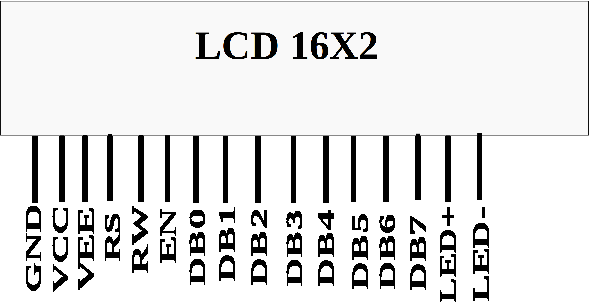
\includegraphics[scale=0.3]{figs/lcd.png} 




\section*{step 6}
-make the Arduino to LCD pin connections as show in  table II
\section*{step 7}
-Open the Arduino IDE and type the following code.Open the serial monitor to enter the inputs

\begin{verbatim}
#include <LiquidCrystal.h>
LiquidCrystal lcd(12,11,5,4,3,2);//arduino pins connected to LCD
int n1,n2;     //initializing input variables
int sum;       //initializing sum variable
void setup()
{
  lcd.begin(16, 2);
  lcd.setCursor(0, 0);
  
  Serial.begin(9600);

  
  //diplaying in serial monitor
  Serial.println("Enter two numbers:");  
  while (Serial.available() == 0)    {}
  //taking first input through serial monitor
  n1= Serial.parseInt();                 
 
  //taking second input through serial monitor
  while (Serial.available() == 0)   {}  
  n2 = Serial.parseInt();

  //required sum
  sum=n1+n2;

  //printing on LCD
  lcd.print("the sum is");
  lcd.setCursor(1,7);
  lcd.print(sum);                     
}
void loop(){
    
  }
 \end{verbatim}


\section*{Result}
-on LCD display you will get the sum of numbers you entered in serial monitor



\end{document}


